% 2010 年山东卷理科第 19 题：五棱锥 P-ABCDE。
% 来源 PDF：普通高考/2010/2010山东理.pdf，SHA-256 c0298cae8fcf19d5f6343a7257702c03f2b618318b10d2340f0c9cc3d67d61f5。
% 原页：第 2 页（A3 三栏）第 1 栏上部，书页码 620。
% 重绘依据：底面 B(0,0)、C(4,0)、A(2,2)、E(4,2)、D(5,1)；P 在 A 上方，PA⊥底面。
%   PA 与 PE 为不可见棱，画虚线；其余棱为实线。
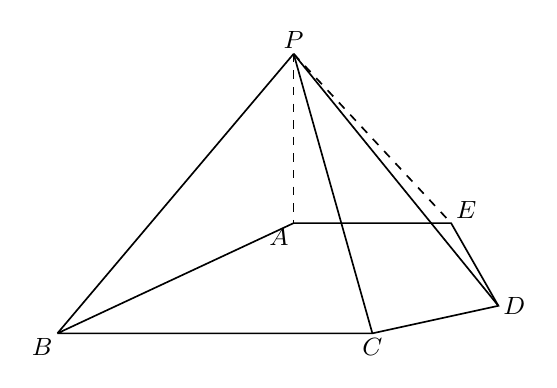
\begin{tikzpicture}[semithick, every node/.style={inner sep=1.5pt, font=\small}]
  \coordinate (B) at (0,0);
  \coordinate (C) at (4,0);
  \coordinate (A) at (3.0,1.4);
  \coordinate (E) at (5.0,1.4);
  \coordinate (D) at (5.6,0.35);
  \coordinate (P) at (3.0,3.55);

  \draw (B) -- (C) -- (D) -- (E) -- (A) -- (B);
  \draw (P) -- (B);
  \draw (P) -- (C);
  \draw (P) -- (D);
  \draw[dashed] (P) -- (A);
  \draw[dashed] (P) -- (E);

  \node[below left] at (B) {$B$};
  \node[below] at (C) {$C$};
  \node[above] at (P) {$P$};
  \node[below left] at (A) {$A$};
  \node[above right] at (E) {$E$};
  \node[right] at (D) {$D$};
\end{tikzpicture}
